\label{sec:intro}

Many real-world sequential-decision making problems involving
resources, time, or spatial configurations naturally use continuous
variables in both their state and action representation and can be
modeled as Hybrid Markov Decision Processes (HMDPs).  While HMDPs have
been studied extensively in the AI
literature~\cite{boyan01,feng04,li05,kveton06,phase07,hao09}, only
recently have symbolic dynamic programming
(SDP)~\cite{sanner_uai11,zamani12} techniques been introduced to
enable the exact solution of multivariate HMDPs with continuous
actions and arbitrary piecewise linear dynamics and rewards.

%% Don't fbox your images... it looks bad... too many extra lines
%% confuse diagram and uneven padding around fbox appears sloppy.

%% DO NOT USED RASTERIZED PNGS!  Reviewers will comment on the
%% graphics not being publication quality!

%%%%%%%%%%%%%%%%%%%%%%%%%%%%%%%%%%%%%%%%%%%%%%%%%%%%%%%%%%%%%%%%%%%%%%%%%%%%%%%%%%%
\begin{figure}[!ht]
\vspace{-2mm}
\centering
\hspace{-5mm}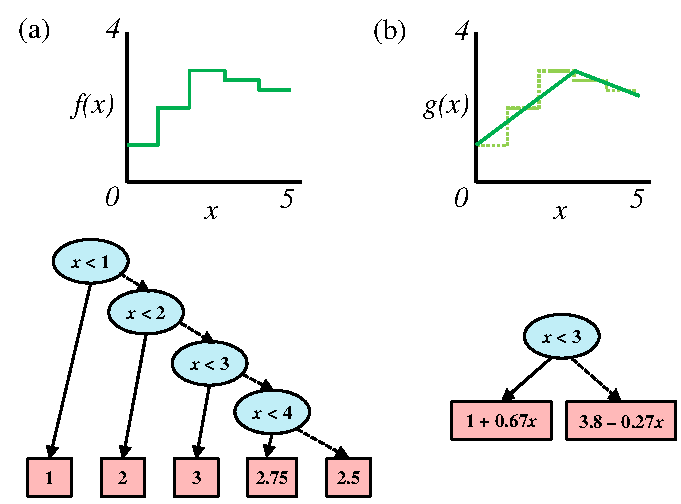
\includegraphics[width=0.45\textwidth]{Figures/xadds/intro_diagram.pdf}
%\subfigure[Step function] {
%	\fbox{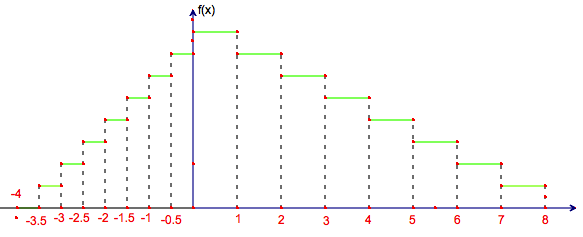
\includegraphics[width=0.45\textwidth]{Figures/stepfun/stepfun.png}}
%	\label{fig:stepf}
%}
%\subfigure[Linear Approximation] {
%	 \fbox{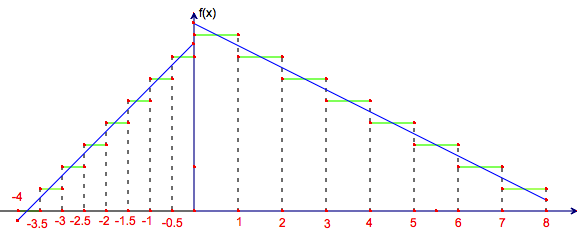
\includegraphics[width=0.45\textwidth]{Figures/stepfun/stepfunapp.png}}
%	\label{fig:steptolin} 
%}
\caption{\footnotesize
(a) A function $f(x)$ for $x \in [0,5]$ and its XADD representation
(solid branch is true, dotted branch is false); (b) A compressed XADD
approximation $g(x)$ of $f(x)$.  While these simple XADDs are trees, XADDs 
are more generally directed acyclic graphs as we show 
later.}  \label{fig:stepfunfig}
\vspace{-3mm}
\end{figure}
%%%%%%%%%%%%%%%%%%%%%%%%%%%%%%%%%%%%%%%%%%%%%%%%%%%%%%%%%%%%%%%%%%%%%%%%%%%%%%%%%%%

What has proved crucial in this SDP solution of piecewise linear HMDPs
is the use of the XADD data structure representation of functions like
the simple examples shown in Figure~\ref{fig:stepfunfig}(a,b) that
allows the HMDP value function to be represented compactly and SDP
operations to be computed efficiently.  In brief, an XADD is simply an
extension of the algebraic decision diagram (ADD)~\cite{bahar93add} to
continuous variables where decisions may be boolean variable tests or
inequalities of continuous expressions and leaves may be continuous
expressions; XADDs are evaluated from root to leaf like decision
trees.  Following the SDP work of~\cite{zamani12} for HMDPs with
continuous actions that we extend, we restrict XADDs to have linear
decisions and leaves.

While XADDs have enabled SDP solutions to HMDPs that would not be
otherwise possible with more na\"{i}ve representations of piecewise
functions, XADDs still have limitations --- for some problems the HMDP
solution (represented by a value function) simply has many distinct
pieces and does not admit a more compact \emph{exact} XADD
representation, e.g, Figure~\ref{fig:stepfunfig}(a).  However,
motivated by previous approximation work in discrete factored MDPs
using ADD approximation~\cite{apricodd}, we pose the question of
whether there exists a method for compressing an XADD in exchange
for some bounded approximation error.  As a hint of the solution, we
note that Figure~\ref{fig:stepfunfig}(a) can be approximated
by \ref{fig:stepfunfig}(b) which is more compact and induces relatively 
small error.  

But how do we find such a compressed XADD?  In the simpler case of
ADDs~\cite{apricodd}, this approximation process was straightforward:
leaves with nearby constant values are averaged and merged, leading to
bottom-up compaction of the ADD.  In the XADD, if we wish to take a
similar approach, we see that the problem is more complex since it is
not clear (1) which leaves to merge, or (2) how to find the best
approximation of these leaves that minimizes the error over the
\emph{constrained, continuous} space where each leaf is valid.  Indeed, as
Figure~\ref{fig:stepfunfig}(a,b) demonstrates, the answer
is \emph{not} given simply by averaging leaves since the average of
constant leaves in (a) could never produce the linear function in the
leaves of (b).  Hence, we wish to answer questions (1) and (2) to
produce a \emph{bounded and low-error approximation over the entire
continuous function domain} like that given in
Figure~\ref{fig:stepfunfig}(b).

To answer these questions, we propose a bounded error compression
technique for linear XADDs that involves the solution of a constrained
bilinear saddle point problem.  Fortuitously, we show that given the
special structure of this problem, it can be expressed as a bilevel
linear programming problem. % (where a constraint itself is an
%optimization problem, leading to a second level of optimization).
While the second-level optimization problem in this
bilevel program implicitly represents an infinite number of
constraints, we show that a constraint generation approach for 
this second stage allows the first stage to terminate at
optimality after generating only a finite number of constraints.  This
solution permits the use of efficient linear program solvers for XADD
compression and enables a novel class of bounded approximate SDP
algorithms for hybrid MDPs.  Empirically we demonstrate that this
approach to XADD compression offers order-of-magnitude speedups over
the exact solution in exchange for a small approximation error, thus
vastly increasing the range of HMDPs for which solutions with strong
error guarantees are possible.

%% No mention of paper organization: this is just filler content that
%% no one ever reads -- readers spot it and skip to the next section.
